\section{Perceptron}
\label{sec:perceptron}

\begin{frame}
  \begin{center}
    \Huge{\textcolor{red}{Perceptron}}
  \end{center}
\end{frame}

\subsection{Perceptron}

\begin{frame}[fragile]{符号}
 \begin{itemize}
   \item \textcolor{red}{Training Set}: $ S = \{ ({x^{(i)}},{y^{(i)}});i = 1,2,...,m\} $
   \item \textcolor{red}{Training Example($i_{th}$)}: $ ({x^{(i)}},{y^{(i)}}) $
   \item \textcolor{red}{Input Variable}: $ x = ({x_1},{x_2},...,{x_n})^{T} \in {\mathbb{R}^n} $
   \item \textcolor{red}{Target Variable}: $ y \in \{0,1\} $
   \item \textcolor{red}{Weights}: $ w = ({w_1},{w_2},...,{w_n})^{T} \in {\mathbb{R}^n} $   
   \item \textcolor{red}{Bias}: $ b \in \mathbb{R} $      
   \item \textcolor{red}{Activation}: $ 
sign(z)= \left\{ \begin{gathered}
  1 \quad z \geqslant 0 \hfill \\
  0 \quad z < 0 \hfill \\ 
\end{gathered}  \right.
$   
 \end{itemize}
\end{frame}

\begin{frame}{感知器}
  \begin{figure}
    \centering
    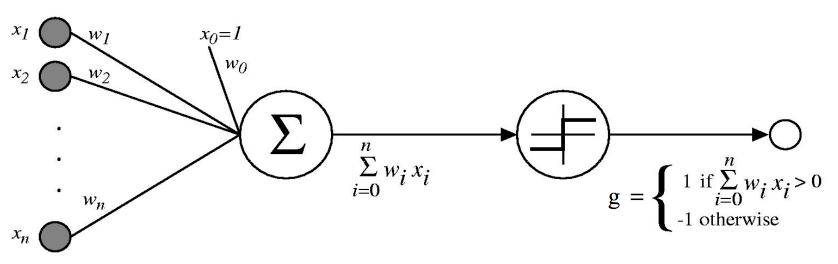
\includegraphics[width=0.8\textwidth]{perceptron.png}
  \end{figure}

\[\begin{gathered}
  {w^T}x = \sum\limits_{i = 0}^n {{w_i}{x_i}}  \hfill \\
  {x_0} = 1 \quad b = {w_0} \hfill \\ 
\end{gathered} \]
\end{frame}

\begin{frame}[fragile]{模型}
\[\begin{gathered}
  y = {h_{w,b}}(x) = sign({w^T}x + b) = \left\{ \begin{gathered}
  1 \quad {w^T}x + b \geqslant 0 \hfill \\
  0 \quad {w^T}x + b < 0 \hfill \\ 
\end{gathered}  \right. \hfill \\
  x = ({x_1},...,{x_n})^{T} \in {\mathbb{R}^n} \quad w = ({w_1},...,{w_n})^{T} \in {\mathbb{R}^n} \hfill \\ 
\end{gathered} \]
\end{frame}

\begin{frame}[fragile]{学习算法}
\[\begin{aligned}
  w \leftarrow  & w - \alpha \left( sign({w^T}x + b) - y \right)x \\ 
  b \leftarrow  & b - \alpha \left( sign({w^T}x + b) - y \right)  \\ 
\end{aligned} \]
\end{frame}


